\section{Diskussion}
Im Rahmen dieser Arbeit wurde ein System zum klassifizieren von Sprachaufnahmen implementiert. Das Programm unterscheidet zwischen Französisch, Deutsch, und Englisch. Mit Deep Learning hat das Programm selbst gelernt die Sprache von kurzen Aufnahmen zu erkennen. Anstatt rohe Schallwellen zu verarbeiten wurden in Echtzeit berechnete Spektrogramme verwendet. Die Spektrogramme konnten mit Bilderkennungsmethoden erfolgreich eingeordnet werden. Ein hybrides Modell aus CNN und RNN besass die höchste Genauigkeit. Die Trainingsdaten wurden wegen fehlenden maßgeschneiderten Datensets aus verschiednen Quellen selbst kompiliert. Es wurde mit Daten von Voxforge und Youtube trainiert um mit Daten aus der Librivox Hörbuchdatenbank getestet zu werden. Die hohe Korrektheit aller Modelle bestätigt, dass tiefe neuronale Netze eine angemessene Methode für Sprachidentifikation sind.
\\ \\
Der Vergleich der Resultate mit anderen Arbeiten ist nur mit Vorsicht möglich. Der wichtigste Unterschied ist, dass andere Daten verwendet werden und dementsprechend nur andere Resultate entstehen können. Glücklicherweise sind Arbeiten zu Automatischer Sprachidentifikation im Internet jedoch frei erhältlich, denn das Problem ist in der Informatik recht jung. Erst in den 70'er Jahren wurde man für das weiterleiten von Telefonanrufen auf das Thema aufmerksam. Eine lange Zeit galt, dass die bessten Systeme diejenigen waren, die die fortgeschrittensten sprachlichen Merkmale berechneten. Der Nachteil an diesen Systemen ist, dass die Erweiterung auf andere Sprachen mit einem grossem Aufwand verbunden ist. \parencite{history}
\\
Erst mit dem Aufkommen von Deep Learning als konkurrenzfähige Methode im letzen Jahrzehnt kamen wieder Systeme mit weniger Preprocessing auf \parencite{chollet}. 2009 erreichte Grégoire Montavon mit Deep Learning für 3 Sprachen auf dem Voxforge Datenset eine Genauigkeit von $80.1\%$ \parencite{montavon}. Das Voxforge Datenset hat sich seither verändert. Es kann angenommen werden, dass die hier vorgestellten Modelle, sein System deutlich übertreffen, da ähnliche Arbeiten dass getestet haben \parencite{iLID}. 2016 wurde mit einem sehr ähnlichen Modell wie das CNN Modell dieser Arbeit Genauigkeiten von 93\% und 85\% für 2 Sprachen respektive 4 Sprachen gemessen \parencite{iLID}. Hrayr et al. \parencite{yerevann} stellen im selben Jahr ein CRNN Modell für einen Wettbewerb vor, dass zwischen 176 Sprachen mit 99.67\% Genauigkeit differenzieren kann. Ein weiteres CRNN Modell von Bartz et al. \parencite{crnn} erreicht 2017 91\% bei der Unterscheidung von vier Sprachen.
\\
Die in dieser Arbeit vorgestellten System leisten vergleichbare Genaugigkeiten wie die genannten Modelle. 95\% ist eine höchst zufriedenstellende Genauigkeit unter anbetracht das das Youtube Datenset nicht fehlerfrei ist. Das Datenset wurde bekanntlich nicht manuell gesäubert. Es können dementsprechend Aufnahmen ohne Sprache oder mit fremdsprachigen Interviews enthalten sein. Der Anteil von fehlerhaften Aufnahmen ist jedoch wahrscheinlich klein. 
Der Fall auf 80\% Genauigkeit beim Librivox Datenset ist normal. Das Modell ist selbstverständlich für die Youtube und Voxforge Daten optimiert und nicht für Hörbücher. Die Librivox Daten haben zum Beispiel unterschiedliche Hintergrundgeräusche und Aufnahmeprotokolle. 80\% bleibt in jedem Fall ein erfreuliches Resultat. Ein Zufallsgenerator würde im Kontrast nur 33\% erreichen. Es kann also aus dem Resultat abgelesen werden, dass das Modell angemessen generalisiert. 
\\ \\
Bis jetzt wurde das Modell nur an öffentlich verfügbaren Daten ausgewertet wo klar war welche Sprache gesprochen wurde. In der Realität soll das Modell aber helfen die Sprache von unbekannten Aufnahmen zu erkennen. In anderen Worten soll das Modell in der Praxis angewendet werden. Dafür wurde ein Interface programmiert wo Benutzer sich selbst Aufnehmen und das Modell damit abfragen können. Das Interface ist in Form einer Webseite auf den Schulservern frei verfügbar. Die meisten Mobilgeräte und Computer sind kompatibel. Abbildung \ref{img:interface} zeigt die Seite nach dem hochladen einer zufälligen Aufnahme.
\begin{figure}[hbt]
	\centering
		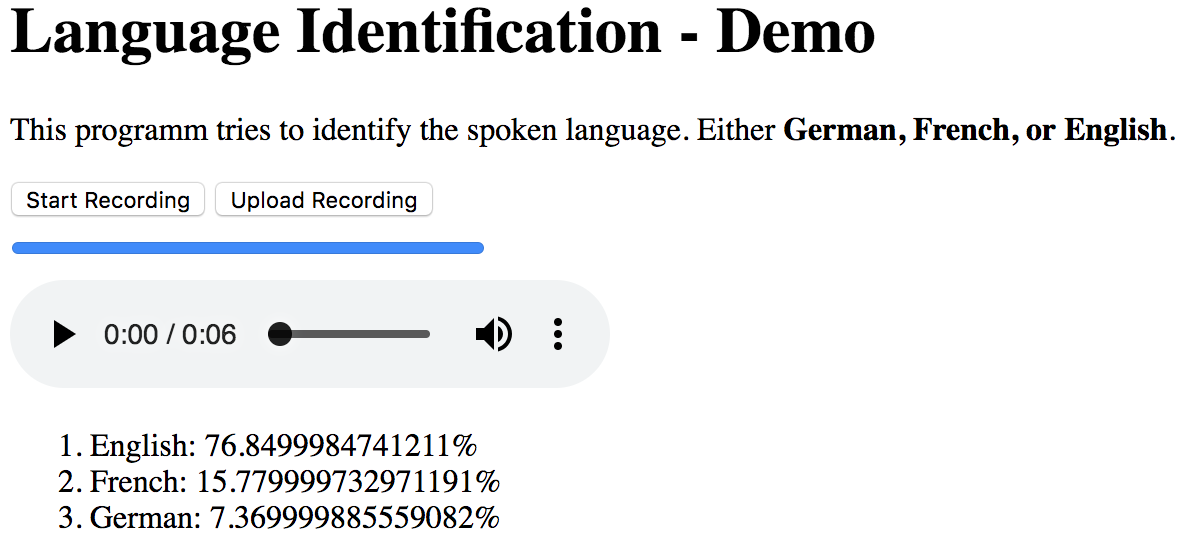
\includegraphics[width=0.6\textwidth]{assets/interface.png}
	\caption{Interface Schnappschuss}
	\label{img:interface}
\end{figure}
Die Umgebung bei Smartphone Aufnahmen ist erneut eine andere wie die von Voxforge und YouTube. Die Genauigkeit die dort erreicht wird ist eine weitere Art die Generalisierbarkeit des Modells zu messen. Aus Neugier wurde ein sehr kleines Datenset aus Aufnahmen von Verwandten und Freunden zusammengestellt. Es wurde darauf geachtet, dass die Sprache deutlich verständlich ist. Insgesamt sind es nur 70 ungleichmässig verteilte Aufnahmen. Die Resultate daraus sind wegen der kleinen Anzahl und Varianz kaum signifikant. Das Programm entdeckt in 70\% der Fälle die richtige Sprache. 
Eine Programm mit Genauigkeit 70\% ist in mancher Hinsicht kein guter Klassifizierer. Kommerziell einsetzbar ist das System damit sicherlich nicht. Für ein Callcenter würde das bedeuten, dass fast jeder dritte Anruf dem falschen Mitarbeiter zugewiesen wird. Das ist aus Sicht der Kunden katastrophal. Also stellt sich die Frage woher der Fehler kommt, bzw. was man noch verbessern kann.
\\ \\
An erster Stelle sind die Daten ein Problem. Die Trainingsdaten sind nicht repräsentativ für alle möglichen Daten, unter anderem Handy-Aufnahmen. Um die Stichprobenverzerrung weiter zu minimieren muss man mehr Daten beschaffen. Die Daten sollten so vielfältig wie möglich sein. Es ist nutzlos unendlich viele Daten zu besitzen wenn die sie sich alle sehr ähnlich sind. Einzelne relevante Merkmale sind unter anderem das Geschlecht, die Stimmhöhe, Hintergrundgeräusche, die Qualität der Aufnahme und die Geschwindigkeit. Je mehr Kombination es gibt desto besser. 
\\
Was macht man aber, wenn man nur eine begrenzte Menge an Daten zur Verfügung hat? In diesem Fall gibt es eine Methode namens \textit{Data Augmentation}. Die Lösung ist, aus den vorhanden Daten weitere Daten zu erschaffen. Manche Merkmale lassen sich nämlich automatisch anpassen. Beispielsweise kann der Computer ohne Problem die Geschwindigkeit und die Qualität der Aufnahme adaptieren. Der Computer passt bei Data Augmentation in jedem Durchlauf zufällig die Merkmale der einzelnen Aufnahmen an. Im Endeffekt wird dem Netzwerk also nie genau die gleiche Aufnahme gezeigt. Das verhindert das das Netzwerk sich an eine endliche Menge von Daten überanpasst. Zudem wird die Stichprobenverzerrung dadurch minimiert. In der Regel hat Data Augmentation immer einen positiven Effekt. Darum ist Data Augmentation  eine mächtige und weit verbreitete Methode.  In dieser Arbeit wurde primär keine Data Augmentation angewendet, weil man die falsche Vorstellung hatte, dass sowieso genug Daten vorhanden wären. Es stellt sich aber im Nachhinein heraus, dass Data Augmentation immer besser ist als dem Netzwerk die gleichen Daten mehrmals zu zeigen. 
\\
An zweiter Stelle sind Mängel beim Training. Die Abbildung mit dem Lernprozess zeigt wie uneben die Kurve der Validation Genauigkeit ist. Manchmal sinkt die Genauigkeit abrupt um im nächsten Durchlauf wieder zu steigen. Die Schwankungen können nur daran liegen, dass das Validationset und das Testset zu klein sind. Das führt dazu, dass sie leicht beeinflussbar sind. Eine Erhöhung auf 25\% der gesamten Daten ist für beide zu empfehlen. Andere Hyperparamter oder ganz andere Modelle könnten ebenfalls besser sein. Allerdings wird für viele Experimente ein leistungsstarker Computer benötigt. Mehr Leistung ist immer hilfreich.
\\
Noch mehr Verbesserungspotenzial liegt wahrscheinlich im Verfahren \textit{Learning from Between-class Examples for Deep Sound Recognition}(2017)\parencite{between}. Yuji et al. stellen eine vielversprechende Methode vor, die die Genauigkeit in jedem ihrer Versuche verbessert. Die Idee ist es, Aufnahmen von verschiedenen Klassen zu kombinieren um eine Mischaufnahme zu erfinden deren Ziel ebenfalls zwischen den Klassen liegt. Vereinfacht angewendet auf Sprachidentifikation könnte das bedeuten, dass eine deutsche und eine französische Aufnahme gleichzeitig abgespielt werden um zu einer Aufnahme kombiniert zu werden. In dieser Aufnahme würden also zwei Sprecher parallel sprechen. Das Ziel der Aufnahme wäre ebenfalls ein Mix z.B $\begin{bmatrix}0.5 & 0 & 0.5 \end{bmatrix}$. Das schöne am Verfahren ist, dass es einfach zu verstehen ist und doch sehr wirksam. Leider reichte die Zeit nicht aus um die Methode zu implementieren.
\\ \\ 
Egal wie viel Potential nach oben am Schluss noch bleibt, war die Arbeit ein Erfolg. Ausser dem Produkt ist immer auch der Weg das Ziel. Es wurde enorm viel gelernt und Erfahrung gesammelt über Deep Learning. Auf der einen Seite zeigt das Projekt wie erstaunlich einfach künstliche Intelligenz in der Praxis ist. Ohne jahrelanges Studium ist man in der Lage das meisste zu verstehen und zu implementieren. Nichts daran ist magisch. In vielerlei Hinsicht ist Deep Learning momentan keine absolute Wissenschaft mit wahr und falsch. Ein grosser Teil der Optimierung besteht aus heuristischen Experimenten. Bei Hyperparametern gibt es noch grossen Forschungsbedarf. Wenn einmal klar ist wie diese gesetzt werden müssen, wird Deep Learning wirklich bereit sein für jedermann. In Zukunft wird es wohl einfachere Inferfaces geben, denen man nur das Problem angeben muss und der Rest automatisch erledigt wird. Auf der anderen Seite ist Deep Learning mathematisch ein kompliziertes Gebiet. Die Grundlagen können in Zukunft nur noch anspruchsvoller werden. Wer wirklich mitforschen will, muss sehr stark in Mathematik sein. Lineare Algebra findet hier tatsächlich Anwendung. Ein ebenfalls nicht zu unterschätzender Teil war das Sammeln und Vorbereiten der Daten. Die Vorstellung man könnte sofort an das Experimentieren ran gehen ist trügerisch. Wenn ein Deep Learning System von null aus aufgebaut wird, spendet man mindestens so viel Zeit bei der Vorbereitung der Daten wie beim Experimentieren. Die wichtige Frage ist wie lange Deep Learning noch so populär bleiben wird. Wird es in ein paar Jahren überhaupt noch relevant sein? Der Nutzen wird auf jedem Fall bleiben während die mediale Aufmerksamkeit wahrscheinlich sinken wird. Es wird gehofft das der Leser etwas nützliches für die Zukunft gelernt hat
